\documentclass[pdflatex,iicol,sn-mathphys-num]{sn-jnl}

\usepackage{amsmath,amssymb,amsthm,mathtools,bm}
\usepackage{booktabs,array,multirow}
\usepackage{float}
\usepackage{graphicx}
\usepackage{xcolor}
\usepackage{microtype}
\usepackage{hyperref}
\usepackage{enumitem}
\usepackage{url}

\setlength{\tabcolsep}{3pt}
\emergencystretch=1em

%% Numbered, captioned algorithm floats built on the already-loaded float
%% package, so no additional class dependency is introduced.
\floatstyle{ruled}
\newfloat{algorithm}{tbp}{loa}
\floatname{algorithm}{Algorithm}

\newtheorem{theorem}{Theorem}[section]
\newtheorem{proposition}[theorem]{Proposition}
\newtheorem{lemma}[theorem]{Lemma}
\newtheorem{corollary}[theorem]{Corollary}
\theoremstyle{definition}
\newtheorem{definition}[theorem]{Definition}
\newtheorem{remark}[theorem]{Remark}

\newcommand{\R}{\mathbb{R}}
\newcommand{\norm}[1]{\left\lVert #1\right\rVert}
\newcommand{\spec}{\operatorname{spec}}
\newcommand{\spr}{\varrho}
\newcommand{\diag}{\operatorname{diag}}
\newcommand{\argmin}{\operatorname*{arg\,min}}
\newcommand{\ii}{\mathrm{i}}
\newcommand{\Ulfa}{U_{\mathrm{LFA}}}
\newcommand{\Ubg}{U_{\mathrm{BG}}}
\newcommand{\Urect}{U_{\mathrm{rect}}}
\newcommand{\Ucmp}{U_{\mathrm{cmp}}}
\newcommand{\Id}{\mathrm{Id}}

\title[Four-Corner Spectral Tuning]{Four-Corner Spectral Tuning for Search-Free ADMM in Diffeomorphic Image Registration}

\author[1]{\fnm{Katherine} \sur{Xie}}
\author[1]{\fnm{Jie} \sur{Wu}}
\author*[1]{\fnm{Xiaohui} \sur{Xie}}\email{xhx@uci.edu}

\affil*[1]{\orgdiv{Department of Computer Science}, \orgname{University of California, Irvine}, \orgaddress{\city{Irvine}, \state{California}, \country{USA}}}

\abstract{The choice of penalty and relaxation parameters strongly affects the
runtime of ADMM-based variational image registration. For a well-posed
quadratic subproblem every admissible pair is already contractive, so the
practical task is to select a rapidly convergent pair without a numerical
spectral search. We show that the rank-one pixelwise registration Hessian and
the scalar Sobolev symbol reduce constant-model tuning exactly to four
curvature--symbol corners, which yields a finite algebraic one-shot predictor.
On all 134 FIRE retinal pairs at $256\times 256$, the predictor reduced median
pairwise runtime by 34.4\% and inner iterations by 39.6\% relative to an
externally validation-selected fixed pair, while landmark error and topology
were unchanged; it was also 51.7\% faster than a safeguarded
Barzilai--Borwein proxy. On ten CIMA histology pairs, matched-protocol runtime
decreased by 20.1\%. Signed variable-coefficient enclosures supply optional
rigorous rate bounds that are not used during tuning.}

\keywords{alternating direction method of multipliers, diffeomorphic image registration, parameter selection, spectral analysis, local Fourier analysis}

\pacs[MSC Classification]{65K10, 65F10, 68U10, 90C25, 65T50}

\begin{document}

\maketitle

\section{Introduction}\label{sec:intro}

Diffeomorphic image registration estimates an invertible, topology-preserving
spatial transformation that aligns a moving image with a fixed image. Classical
variational methods remain attractive because they provide explicit control
over the deformation model, the regularization, and the numerical stopping
criteria, and because they can be applied without training data. Representative
approaches include DARTEL, diffeomorphic demons, large-deformation
optimal-control formulations, and modern GPU-accelerated variational solvers
\cite{Ashburner2007,Vercauteren2009,MangBiros2015,Thorley2021}. Even as
learning-based registration has matured \cite{Hering2022}, the main practical
limitation of these classical solvers remains computational cost.

Many diffeomorphic schemes update a velocity field through a sequence of
convex, linearized optical-flow problems. A typical quadratic subproblem is
\begin{equation}
\min_{v=(v_x,v_y)}
\frac{\mu}{2}\norm{I_x\odot v_x+I_y\odot v_y+I_t}_2^2
+\frac{1}{2}\norm{Lv}_2^2,
\label{eq:registration}
\end{equation}
where $\mu>0$ is a data-fidelity weight, $I_x$ and $I_y$ are spatial image
derivatives, $I_t$ is the current temporal or residual derivative, $\odot$
denotes the pointwise product, and $L$ is a differential regularization
operator. Splitting the data and
regularization terms produces inexpensive pixelwise and Fourier-domain
subproblems, which makes ADMM particularly suitable for GPU implementation
\cite{Thorley2021,Song2024}.

In this splitting, the ADMM penalty $\rho>0$ scales the quadratic constraint
term that couples the data and regularization subproblems, while the
over-relaxation parameter $\alpha\in(0,2]$ mixes the most recent primal update
into the dual and secondary steps; both strongly affect the iteration's
contraction rate and therefore the practical runtime.
Fixed defaults, residual balancing, and adaptive spectral rules can all be
effective, but none of them exploits the unusually specific geometry of
registration: the data Hessian is block diagonal with rank-one $2\times2$
blocks, whereas the regularizer is a scalar elliptic operator applied
identically to each velocity component. General quadratic ADMM theory yields
optimal parameters for several special classes
\cite{Ghadimi2015,Teixeira2016,GiselssonBoyd2017}. More recently, Song et al.
optimized $\rho$ numerically for general linear quadratic problems and derived
an optimal $\alpha$ conditional on $\rho$, including experiments on
diffeomorphic registration \cite{Song2024}; their registration penalty still
requires a spectral optimization.

Our approach is based on local Fourier analysis (LFA), a classical tool for
predicting and optimizing stationary iterations for constant-coefficient
differential operators \cite{ChanElman1989,WienandsJoppich2005}. Standard LFA
is exact for translation-invariant periodic problems, and nonstandard variants
remain predictive for jumping and random coefficients
\cite{Kumar2019,Rodrigo2017}. The rank-one image-gradient blocks admit a
sharper global reduction: the constant-model tuning envelope depends only on
the two attained data-curvature endpoints and the two attained
regularizer-symbol endpoints. This yields four branches, a finite algebraic
candidate set, and no numerical search over the penalty.

\paragraph{Contributions.}
\begin{enumerate}[leftmargin=1.6em,itemsep=2pt,topsep=3pt]
\item An exact reduced Cayley representation and a strict-contraction
characterization for well-posed quadratic registration subproblems
(Section~\ref{sec:reduced}).
\item An exact four-corner reduction and a finite algebraic, search-free joint
predictor for rank-one registration Hessians
(Sections~\ref{sec:fourcorner} and \ref{sec:selection}).
\item Optional signed variable-coefficient rate enclosures for nonnormal
iterations (Section~\ref{sec:certification}).
\item FIRE and CIMA validation demonstrating lower end-to-end runtime at
matched landmark accuracy and topology (Section~\ref{sec:results}).
\end{enumerate}

\paragraph{Organization.}
Section~\ref{sec:related} reviews related work. Section~\ref{sec:model} fixes
the discrete registration model and the ADMM splitting, and
Section~\ref{sec:reduced} derives the exact reduced iteration.
Section~\ref{sec:fourcorner} establishes the four-corner reduction,
Section~\ref{sec:certification} develops the optional rate certificates, and
Section~\ref{sec:selection} gives the finite parameter selector.
Sections~\ref{sec:protocol} and \ref{sec:results} describe the implementation
and the experiments; Sections~\ref{sec:discussion} and \ref{sec:conclusion}
discuss the findings and conclude.

\section{Related Work}\label{sec:related}

\subsection{ADMM parameter selection}
The scaled ADMM iteration and its practical residual stopping criteria were
systematized by Boyd et al. \cite{Boyd2011}. Ghadimi et al. derived optimal
penalties and relaxation parameters for several quadratic classes
\cite{Ghadimi2015}, and Teixeira et al. studied scaling, preconditioning, and
optimal ADMM parameters in distributed quadratic programming
\cite{Teixeira2016}. Giselsson and Boyd developed tight contraction bounds and
metric selection for Douglas--Rachford splitting and ADMM under
strong-convexity and smoothness assumptions \cite{GiselssonBoyd2017}. Adaptive
alternatives include residual balancing and Barzilai--Borwein (BB) type
spectral updates \cite{Wohlberg2017,Xu2017}.

The closest work is that of Song et al. \cite{Song2024}, who formulate ADMM and
over-relaxed ADMM (oADMM) for general linear quadratic problems, optimize the
penalty from the iteration spectrum, give a closed-form relaxation parameter
for a fixed penalty, and include diffeomorphic image registration as an
application. Our objective differs in kind. Instead of a full-spectrum
criterion for a general quadratic program, we exploit the specific geometry of
a rank-one registration data term paired with a scalar Sobolev regularizer.
That geometry replaces their numerical one-variable spectral optimization of
the penalty by a finite four-corner predictor, and their conditional relaxation
formula by a finite set of piecewise-linear candidates; neither stage requires
gradient descent, repeated ADMM trials, or the full iteration spectrum. Spatial
coefficient variation is likewise treated differently: rather than forming the
exact spectrum of the full iteration, we combine a local predictor with a
separately evaluated signed enclosure that assumes no commutativity. The
resulting selector is assessed empirically by matched-accuracy runtime
reductions on the FIRE and CIMA landmark benchmarks.

\subsection{ADMM and variational diffeomorphic registration}
DARTEL \cite{Ashburner2007} and diffeomorphic demons \cite{Vercauteren2009} are
influential optimization-based registration methods. Thorley et al. proposed a
fast diffeomorphic method that composes nonstationary velocity updates and
solves arbitrary-order regularized convex subproblems with accelerated ADMM on
GPUs \cite{Thorley2021}. Song et al. later used a closely related quadratic
registration model to evaluate spectrally optimized ADMM and oADMM
\cite{Song2024}.

\subsection{Local Fourier analysis}
Fourier analysis has long been used to estimate convergence factors of
stationary iterations for elliptic problems \cite{ChanElman1989}, and LFA
became a principal tool for multigrid design and parameter optimization
\cite{WienandsJoppich2005}. Its exactness under periodic translation-invariant
assumptions, and its extensions to broader settings, have been studied
theoretically \cite{Rodrigo2017}, and nonstandard LFA accurately predicts
multigrid behavior for random and discontinuous coefficients \cite{Kumar2019}.
Our use of LFA differs in two respects: the iteration is an ADMM splitting map
rather than a smoother, and the variable coefficient is a matrix-valued,
rank-one optical-flow Hessian.

\section{Registration Model and ADMM Splitting}\label{sec:model}

\subsection{Discrete quadratic model}
Let the image domain contain $n$ grid points in dimension $d\in\{2,3\}$, let
$\Delta x$ denote the grid spacing, and stack the $d$ velocity components into
$v\in\R^{dn}$. Write $I$ for the linearized image intensity and, at grid point
$x_i$, let $q_i=\nabla I(x_i)\in\R^d$ be its spatial gradient. With data weight
$\mu>0$, and allowing an optional isotropic damping $\nu\ge0$ already present in
some implementations, the linearized data Hessian is the block-diagonal matrix
\begin{equation}
\begin{gathered}
H=\diag\!\left(H_1,\ldots,H_n\right),\\
H_i=\nu I_d+\mu q_iq_i^\top\succeq0.
\end{gathered}
\label{eq:H}
\end{equation}
When $\nu=0$ this recovers the pure rank-one optical-flow Hessian. Each
$d\times d$ block has eigenvalues $\nu$ (with multiplicity $d-1$) and
$\nu+\mu\norm{q_i}^2$. Throughout, $\Id$ denotes the identity of conforming
size on $\R^{dn}$ unless a subscript such as $I_d$ or $I_n$ indicates
otherwise.

We assume a componentwise Sobolev regularizer. Let $G_0\in\R^{n\times n}$ be a
symmetric positive semidefinite discretization of a scalar elliptic operator on
the $n$-point grid (finite-difference or spectral), and let $I_d$ denote the
$d\times d$ identity. The full regularizer on the stacked velocity is then the
Kronecker product
\begin{equation}
G=L^\top L=G_0\otimes I_d\in\R^{dn\times dn},
\label{eq:G}
\end{equation}
which applies the same spatial operator $G_0$ independently to each of the $d$
velocity components; equivalently, $L$ is a differential regularization
operator acting componentwise. A small zeroth-order term $\gamma I_n$, with
weight $\gamma\ge0$ and $I_n$ the $n\times n$ identity, or an appropriate
boundary condition, may be included in $G_0$ to remove its common nullspace.

When $G_0$ is translation-invariant and periodic, it is diagonalized by the
discrete Fourier transform. Its eigenvalues are then given by a scalar Fourier
symbol $g(\xi)$, indexed by discrete frequencies $\xi\in\R^d$. For a first-order
Sobolev regularizer with stiffness $\beta>0$,
\begin{equation}
g(\xi)=\gamma+\frac{4\beta}{(\Delta x)^2}\sum_{\ell=1}^{d}\sin^2\!\left(\frac{\xi_\ell}{2}\right).
\label{eq:regularizer_symbol}
\end{equation}
Thus $\spec(G_0)=\{g(\xi)\}$ over the discrete frequencies, and
$\spec(G)=\spec(G_0)$ with multiplicity $d$. In particular, the spectral
endpoints used later satisfy
$g_-=\lambda_{\min}(G_0)=\min_\xi g(\xi)$ and
$g_+=\lambda_{\max}(G_0)=\max_\xi g(\xi)$.

The registration subproblem is
\begin{equation}
\min_v\;\tfrac12 v^\top Hv+b^\top v+\tfrac12v^\top Gv,
\label{eq:quadratic}
\end{equation}
where $b\in\R^{dn}$ stacks the linearized optical-flow residuals (in two
dimensions, the $i$th block is proportional to $\mu I_t(x_i)\,q_i$, up to sign
convention). We split \eqref{eq:quadratic} by introducing an auxiliary copy
$w=v$:
\begin{equation}
\begin{gathered}
\min_{v,w}\;f_H(v)+f_G(w)
\quad\text{subject to}\quad v-w=0,\\
f_H(v):=\tfrac12v^\top Hv+b^\top v,
\qquad
f_G(w):=\tfrac12w^\top Gw.
\end{gathered}
\label{eq:split}
\end{equation}

\subsection{ADMM and over-relaxation}
Let $u\in\R^{dn}$ denote the scaled dual variable associated with the
constraint $v-w=0$. Standard ADMM applied to \eqref{eq:split} is
\begin{align}
(H+\rho\Id)v^{k+1}&=-b+\rho(w^k-u^k),\label{eq:vupdate}\\
(G+\rho\Id)w^{k+1}&=\rho(v^{k+1}+u^k),\label{eq:wupdate}\\
u^{k+1}&=u^k+v^{k+1}-w^{k+1}.\label{eq:uupdate}
\end{align}
For oADMM, $v^{k+1}$ is replaced in the $w$ and dual updates by
\begin{equation}
\widehat v^{k+1}=\alpha v^{k+1}+(1-\alpha)w^k,
\qquad 0<\alpha\le2 .
\label{eq:relaxed}
\end{equation}
The linear term $b$ shifts the fixed point but does not affect error
propagation, so all spectral statements below concern the homogeneous
iteration. We write $T_{\rho,\alpha}$ for the resulting linear error map on the
state $(w,u)$, defined by the homogeneous form of
\eqref{eq:vupdate}--\eqref{eq:uupdate} with the relaxation
\eqref{eq:relaxed}.

\section{Exact Reduced Iteration}\label{sec:reduced}

Define the resolvents and Cayley transforms
\begin{align}
P_H(\rho)&=\rho(H+\rho\Id)^{-1},\\
C_H(\rho)&=(H-\rho\Id)(H+\rho\Id)^{-1}=\Id-2P_H(\rho),\\
P_G(\rho)&=\rho(G+\rho\Id)^{-1},\\
C_G(\rho)&=(G-\rho\Id)(G+\rho\Id)^{-1}=\Id-2P_G(\rho).
\end{align}

\begin{proposition}[Reduced Cayley iteration]\label{prop:reduced}
For the quadratic splitting \eqref{eq:split}, all nonzero eigenvalues of the
standard ADMM error matrix $T_{\rho,1}$ coincide with the eigenvalues of
\begin{equation}
E_{\rho,1}=\tfrac12\left(\Id+C_H(\rho)C_G(\rho)\right).
\label{eq:Estandard}
\end{equation}
For oADMM the corresponding reduced operator is
\begin{equation}
E_{\rho,\alpha}
=\left(1-\frac{\alpha}{2}\right)\Id
+\frac{\alpha}{2}C_H(\rho)C_G(\rho),
\label{eq:Ealpha}
\end{equation}
and consequently $\spr(T_{\rho,\alpha})=\spr(E_{\rho,\alpha})$, where $\spr$
denotes the spectral radius.
\end{proposition}

The proof is given in Appendix~\ref{app:reduced}. The product $C_HC_G$ is
generally nonnormal because $H$ and $G$ do not commute, which is precisely why
a global simultaneous diagonalization is unavailable for registration.

\begin{theorem}[Contraction is independent of tuning]\label{thm:basic-contraction}
Let $H,G\succeq0$ and $H+G\succ0$. For every $\rho>0$,
\begin{equation}
\kappa_\rho:=\norm{C_H(\rho)C_G(\rho)}_2<1 .
\end{equation}
Consequently, for every $0<\alpha\le2$,
\begin{equation}
\spr(E_{\rho,\alpha})\le\norm{E_{\rho,\alpha}}_2
\le1-\frac{\alpha}{2}\left(1-\kappa_\rho\right)<1 .
\end{equation}
\end{theorem}

\begin{proof}
For a symmetric positive semidefinite matrix $A$, the Cayley eigenvalue at
$\lambda\ge0$ is $(\lambda-\rho)/(\lambda+\rho)$, whose modulus is at most one,
with equality only at $\lambda=0$. Thus $\norm{C_Ax}_2\le\norm{x}_2$, with
equality exactly when $x\in\ker A$. If equality held for $C_HC_G$ on a unit
vector $x$, then equality in both inequalities
$\norm{C_HC_Gx}_2\le\norm{C_Gx}_2\le\norm{x}_2$ would give $x\in\ker G$, hence
$C_Gx=-x$ and $C_Gx\in\ker H$. Therefore $x\in\ker H\cap\ker G$, contradicting
$H+G\succ0$. Compactness of the unit sphere gives $\kappa_\rho<1$. The oADMM
bound follows from the triangle inequality applied to \eqref{eq:Ealpha}, whose
coefficients are nonnegative for $0<\alpha\le2$.
\end{proof}

\paragraph{Nullspaces and conventions.}
If a nonzero $x$ lies in both kernels, then $C_Hx=C_Gx=-x$, $C_HC_Gx=x$, and
$E_{\rho,\alpha}x=x$. This is a direction along which the objective is
nonunique, not a tuning-induced instability. Registration removes it by
zeroth-order regularization, by appropriate boundary conditions, or by
restriction to the identifiable subspace. The endpoint $\alpha=2$ is admissible
for the reduced linear contraction above; implementations whose standard oADMM
theorem assumes $\alpha<2$ should retain that conventional restriction.

\section{Four-Corner Spectral Tuning}\label{sec:fourcorner}

\subsection{Patch surrogate}
Partition the image grid into $R$ patches $\{\Omega_r\}_{r=1}^{R}$. On patch $r$,
choose a representative image-gradient Hessian
\begin{equation}
H_r=\mu\,\bar q_r\bar q_r^\top+\nu I_d,
\label{eq:Hr}
\end{equation}
where $\bar q_r$ may be a center, mean, or robust medoid gradient and $\nu\ge0$
is the optional damping from \eqref{eq:H}.
Denote its eigenvalues by $h_{r,1}\le\cdots\le h_{r,d}$; for the rank-one model,
$h_{r,1}=\cdots=h_{r,d-1}=\nu$ and $h_{r,d}=\nu+\mu\norm{\bar q_r}^2$.

Let $G_r$ be a translation-invariant patch regularizer, implemented with
periodic patch boundary conditions or another transform-diagonalizable closure,
and write $g_r(\xi)$ for its scalar Fourier symbol. Define the attained symbol
endpoints
\begin{equation}
g_r^-:=\min_\xi g_r(\xi),\qquad g_r^+:=\max_\xi g_r(\xi),
\end{equation}
so that $g_r(\xi)\in[g_r^-,g_r^+]$. The block-direct-sum surrogate is
\begin{equation}
\widetilde H=\bigoplus_r\left(I_{|\Omega_r|}\otimes H_r\right),
\qquad
\widetilde G=\bigoplus_r\left(G_r\otimes I_d\right).
\end{equation}
We write $\widetilde E_{\rho,\alpha}$ for the reduced oADMM operator
\eqref{eq:Ealpha} formed with $(\widetilde H,\widetilde G)$ in place of
$(H,G)$.

\subsection{Exact patch symbol}
Because $H_r$ acts only on velocity components while $G_r$ has a scalar spatial
symbol, the two commute on a patch. This gives the frozen-patch spectrum in
closed form.

\begin{theorem}[Frozen-patch spectrum]\label{thm:frozen}
The reduced oADMM surrogate $\widetilde E_{\rho,\alpha}$ is normal, and its
eigenvalues are
\begin{equation}
e_{r,j}(\xi;\rho,\alpha)
=1-\frac{\alpha}{2}
+\frac{\alpha}{2}\,
\frac{h_{r,j}-\rho}{h_{r,j}+\rho}\,
\frac{g_r(\xi)-\rho}{g_r(\xi)+\rho}.
\label{eq:local_eig}
\end{equation}
Equivalently, writing
\begin{equation}
\theta(h,g;\rho)=\frac{\rho^2+hg}{(\rho+h)(\rho+g)},
\label{eq:theta}
\end{equation}
we have $e_{r,j}(\xi;\rho,\alpha)=1-\alpha+\alpha\,\theta(h_{r,j},g_r(\xi);\rho)$,
so that the exact frozen-patch envelope is
\begin{equation}
\Ulfa(\rho,\alpha)=\max_{r,j,\xi}\left|e_{r,j}(\xi;\rho,\alpha)\right|.
\label{eq:ULFA}
\end{equation}
\end{theorem}

\subsection{Corner reduction}
The continuous maximization over frequency in \eqref{eq:ULFA} is unnecessary.

\begin{lemma}[Corner principle]\label{lem:corners}
For fixed $\rho>0$ and scalar arguments $h,g\ge0$,
\begin{equation}
\begin{aligned}
\frac{\partial\theta}{\partial h}
&=\frac{\rho(g-\rho)}{(g+\rho)(h+\rho)^2},\\
\frac{\partial\theta}{\partial g}
&=\frac{\rho(h-\rho)}{(h+\rho)(g+\rho)^2}.
\end{aligned}
\end{equation}
Hence $\theta$ is coordinatewise monotone on every rectangle
$[h^-,h^+]\times[g^-,g^+]$, and its extrema occur at the four corners. Since
$|1-\alpha+\alpha\theta|$ is convex as a function of $\theta$, its maximum also
occurs at a corner. In the present setting the second argument ranges over
regularizer eigenvalues, i.e.\ values of the symbol $g(\xi)$ or, equivalently,
of $\spec(G_0)$.
\end{lemma}

\begin{theorem}[Global four-corner reduction]\label{thm:global_four}
Let $H_i=\nu I_d+\mu q_iq_i^\top$ as in \eqref{eq:H}, let
$g_-=\lambda_{\min}(G_0)$ and $g_+=\lambda_{\max}(G_0)$ be the attained extrema
of the discrete scalar regularizer spectrum, and put
\begin{equation}
h_-=\nu,\qquad h_+=\nu+\mu\max_i\norm{q_i}^2 .
\label{eq:hpm}
\end{equation}
For every $\rho>0$ and every $0<\alpha\le2$, the envelope over all pixelwise
rank-one curvatures and all regularizer frequencies equals
\begin{equation}
\max_{(h,g)\in\{h_-,h_+\}\times\{g_-,g_+\}}
\left|1-\alpha+\alpha\,\theta(h,g;\rho)\right|.
\label{eq:four_corner_envelope}
\end{equation}
Consequently the finite joint constant-model predictor depends on exactly four
branches, independently of image size and of the number of distinct gradient
magnitudes.
\end{theorem}

\begin{proof}
Every data eigenvalue equals either $\nu$ or $\nu+\mu\norm{q_i}^2$, hence lies
in $[h_-,h_+]$, and both endpoints are attained: the lower endpoint corresponds
to the direction orthogonal to $q_i$. By Lemma~\ref{lem:corners}, $\theta$ maps
the rectangle $[h_-,h_+]\times[g_-,g_+]$ onto an interval whose endpoints are
attained at its corners. The map $t\mapsto|1-\alpha+\alpha t|$ is convex, so its
maximum over that interval is attained at an endpoint, and therefore at one of
the same four corners. The argument permits $h_-=0$, $g_-=0$, repeated
endpoints, and common nullspaces, because every denominator in
\eqref{eq:theta} is strictly positive for $\rho>0$.
\end{proof}

More generally, for the patchwise surrogate let
\begin{equation}
\mathcal C=\bigcup_{r,j}
\left\{(h_{r,j},g_r^-),(h_{r,j},g_r^+)\right\}.
\label{eq:cornerset}
\end{equation}
Then
\begin{equation}
\Ulfa(\rho,\alpha)
=\max_{(h,g)\in\mathcal C}
\left|1-\alpha+\alpha\,\theta(h,g;\rho)\right|,
\label{eq:finite_envelope}
\end{equation}
so the full local Fourier calculation reduces to a small finite set even in
three dimensions. For the global rank-one predictor,
Theorem~\ref{thm:global_four} sharpens this set to four entries; patchwise sets
remain useful only when a local rather than a global model is deliberately
constructed.

\section{Optional Variable-Coefficient Rate Certification}\label{sec:certification}

This section develops rigorous upper bounds on the contraction factor of the
full variable-coefficient iteration. The bounds are optional diagnostics: they
are evaluated once, after the fact, at the parameters chosen in
Section~\ref{sec:selection}, and they play no role in the timed registration
algorithm. A reader interested only in the practical method may proceed
directly to Section~\ref{sec:selection}.

\subsection{Frozen-patch perturbation certificate}
We first retain the frozen-patch perturbation certificate as a rigorous but
deliberately conservative baseline. It replaces both $H$ and $G$ by their patch
surrogates. Define
\begin{equation}
\begin{gathered}
\delta_H=\norm{H-\widetilde H}_2,
\qquad
\delta_G=\norm{G-\widetilde G}_2,\\
\delta=\delta_H+\delta_G .
\end{gathered}
\label{eq:deltas}
\end{equation}
For block-diagonal $H$, the quantity $\delta_H$ is the largest patchwise
$2$-norm of a $d\times d$ block difference and is therefore inexpensive. The
regularizer error $\delta_G$ can be computed with a few power iterations, or
bounded by a row-sum estimate of the patch-boundary stencil discrepancy.

\begin{lemma}[Cayley Lipschitz bound]\label{lem:cayley_lipschitz}
For symmetric positive semidefinite $A,B$ and $\rho>0$,
\begin{equation}
\norm{C_A(\rho)-C_B(\rho)}_2\le\frac{2}{\rho}\norm{A-B}_2 .
\label{eq:cayley_lipschitz}
\end{equation}
\end{lemma}

\begin{theorem}[Certified local spectral envelope]\label{thm:certified}
Let $\Ulfa$ be defined by \eqref{eq:finite_envelope}. Then, for $0<\alpha\le2$,
\begin{equation}
\spr(T_{\rho,\alpha})
\le
\mathcal U(\rho,\alpha)
:=\Ulfa(\rho,\alpha)+\frac{\alpha\delta}{\rho}.
\label{eq:certified_envelope}
\end{equation}
No commutativity assumption on the full matrices $H$ and $G$ is required.
\end{theorem}

The proof is given in Appendix~\ref{app:perturbation}. The bound separates two
effects: $\Ulfa$ measures the exact contraction of the frozen local models,
while $\alpha\delta/\rho$ penalizes spatial coefficient variation and
patch-boundary approximation. A larger $\rho$ suppresses the perturbation term,
whereas an excessively large $\rho$ worsens the local Cayley balance. This
tradeoff makes parameter selection nontrivial and certifiable.

\begin{corollary}[Guaranteed convergence]\label{cor:convergence}
If the selected parameters satisfy $\mathcal U(\rho,\alpha)<1$, then the full
linearized registration ADMM/oADMM iteration converges linearly with asymptotic
factor at most $\mathcal U(\rho,\alpha)$.
\end{corollary}

\subsection{Signed enclosures with the exact regularizer}
We now retain $G=G_0\otimes I_d$ exactly. Let
\begin{equation}
K_\rho:=(G_0-\rho I_n)(G_0+\rho I_n)^{-1}\in\R^{n\times n}
\end{equation}
be the scalar Cayley transform of $G_0$, so that $C_G(\rho)=K_\rho\otimes I_d$.
Write $C_H=\diag(C_1,\ldots,C_n)$, where each
$C_i=(H_i-\rho I_d)(H_i+\rho I_d)^{-1}$ is an explicit symmetric $d\times d$
block, so that $(C_HC_G)_{ij}=(K_\rho)_{ij}C_i$. Throughout this subsection set
\begin{equation}
\begin{gathered}
B^S_{ij}=|(K_\rho)_{ij}|\,\norm{(C_i+C_j)/2}_2,\\
B^Q_{ij}=|(K_\rho)_{ij}|\,\norm{(C_i-C_j)/2}_2
\end{gathered}
\label{eq:comparison_matrices}
\end{equation}
for $i\ne j$, with zero diagonal, and let $d_i^-$ and $d_i^+$ denote the
extreme eigenvalues of the normal diagonal block $(K_\rho)_{ii}C_i$. Collect
these scalars into the vectors
$d^\pm:=(d_1^\pm,\ldots,d_n^\pm)\in\R^n$.

\begin{theorem}[Block-Gershgorin enclosure]\label{thm:block_gershgorin}
Every eigenvalue of $C_HC_G$ lies in a disk
\begin{equation}
\left|z-(K_\rho)_{ii}c_{i,r}\right|
\le\norm{C_i}_2\sum_{j\ne i}\left|(K_\rho)_{ij}\right|
\end{equation}
for some pixel $i$ and some eigenvalue $c_{i,r}$ of $C_i$. The resulting affine
disk envelope
\begin{equation}
\begin{aligned}
\Ubg(\rho,\alpha)=\max_{i,r}\Big[
&\left|1-\tfrac{\alpha}{2}+\tfrac{\alpha}{2}(K_\rho)_{ii}c_{i,r}\right|\\[-2pt]
&+\tfrac{\alpha}{2}\norm{C_i}_2\sum_{j\ne i}\left|(K_\rho)_{ij}\right|
\Big]
\end{aligned}
\end{equation}
is a rigorous upper bound on $\spr(T_{\rho,\alpha})$.
\end{theorem}

\begin{proof}[Proof sketch]
Select the eigenvector block of maximum Euclidean norm. The diagonal block
$(K_\rho)_{ii}C_i$ is normal, so its shifted smallest singular value is exactly
the distance to its spectrum, and the off-diagonal block row supplies the
stated radius. The affine oADMM scaling in \eqref{eq:Ealpha} transfers the disk
enclosure to $T_{\rho,\alpha}$.
\end{proof}

The same block structure yields a signed rectangle, which is sharper because it
retains the sign of the real part. Writing $M:=C_HC_G$, let
$S=(M+M^\top)/2$ and $Q=(M-M^\top)/2$ denote its Hermitian and skew-Hermitian
parts, whose off-diagonal blocks are
\begin{equation}
S_{ij}=(K_\rho)_{ij}\frac{C_i+C_j}{2},
\qquad
Q_{ij}=(K_\rho)_{ij}\frac{C_i-C_j}{2},
\end{equation}
and define
\begin{align}
m_\rho&=\min_i\Big[d_i^--\textstyle\sum_{j\ne i}B^S_{ij}\Big],
\label{eq:mrho}\\
M_\rho&=\max_i\Big[d_i^++\textstyle\sum_{j\ne i}B^S_{ij}\Big],
\label{eq:Mrho}\\
\eta_\rho&=\max_i\textstyle\sum_{j\ne i}B^Q_{ij}.
\label{eq:etarho}
\end{align}

\begin{theorem}[Commutator-aware rectangle]\label{thm:rectangle}
The spectrum satisfies
$\spec(C_HC_G)\subset[m_\rho,M_\rho]+\ii\,[-\eta_\rho,\eta_\rho]$, and therefore
\begin{equation}
\begin{gathered}
\spr(T_{\rho,\alpha})\le\Urect:=\max_{x\in\{m_\rho,M_\rho\}}\Phi(x),\\
\Phi(x)=\sqrt{\left(1-\tfrac{\alpha}{2}+\tfrac{\alpha x}{2}\right)^{2}
+\left(\tfrac{\alpha\eta_\rho}{2}\right)^{2}} .
\end{gathered}
\label{eq:Urect}
\end{equation}
For fixed $\rho$, the minimizing $\alpha$ is an endpoint of the admissible
interval, a stationary point of either quadratic under the square root, or the
intersection $4/(2-m_\rho-M_\rho)$ when that value is admissible.
\end{theorem}

\begin{proof}[Proof sketch]
Real parts of eigenvalues lie in the Rayleigh interval of $S$, and imaginary
parts are bounded by $\norm{Q}_2$. Hermitian block-Gershgorin estimates bound
$S$, while the symmetric matrix of block norms bounds $\norm{Q}_2$ by its
maximum row sum. Note that $\eta_\rho=0$ for constant data blocks, in which case
the rectangle degenerates to a real interval.
\end{proof}

The row maxima in \eqref{eq:mrho}--\eqref{eq:etarho} can be replaced by a
strictly stronger global comparison construction.

\begin{theorem}[Perron comparison rectangle]\label{thm:comparison}
Theorem~\ref{thm:rectangle} remains valid with
\begin{equation}
\begin{gathered}
m_\rho=\lambda_{\min}\!\left(\diag(d^-)-B^S\right),\\
M_\rho=\lambda_{\max}\!\left(\diag(d^+)+B^S\right),\\
\eta_\rho=\spr(B^Q).
\end{gathered}
\label{eq:perron}
\end{equation}
These bounds are never weaker than their block-row-sum counterparts. They
require three symmetric scalar $n\times n$ eigenproblems and never form the
$dn\times dn$ iteration matrix. We write $\Ucmp(\rho,\alpha)$ for the value of
\eqref{eq:Urect} obtained from \eqref{eq:perron}.
\end{theorem}

\begin{proof}[Proof sketch]
For a block vector $x$, set $y_i=\norm{x_i}_2$. Bounding each Hermitian
quadratic cross term by $B^S_{ij}y_iy_j$ gives the two scalar Rayleigh
quotients. The same block-norm comparison gives $\norm{Qx}_2\le\norm{B^Qy}_2$,
hence $\norm{Q}_2\le\norm{B^Q}_2=\spr(B^Q)$. Standard bounds of eigenvalues by
maximum row sums prove dominance over the earlier rectangle.
\end{proof}

\begin{corollary}[Sparse truncated-kernel certificate]\label{cor:truncated_kernel}
Assume periodic boundaries, so that $K_\rho$ is the convolution operator on the
$n$-point grid associated with a scalar kernel $k_\rho$, indexed by discrete
spatial offsets $s$. Retain offsets in a finite stencil $\mathcal R$, write
$K_{\rho,\mathcal R}$ for the truncated convolution that keeps only those
offsets, define the omitted tail
$\tau_{\mathcal R}=\sum_{s\notin\mathcal R}|k_\rho(s)|$, and construct the
comparison rectangle of Theorem~\ref{thm:comparison} from the retained offsets
only, giving $U_{\mathcal R}$. Then
\begin{equation}
\spr(T_{\rho,\alpha})\le U_{\mathcal R}
+\frac{\alpha}{2}\max_i\norm{C_i}_2\,\tau_{\mathcal R}.
\end{equation}
For a fixed-radius stencil the comparison matrices are sparse, FFT evaluation
of $k_\rho$ costs $O(n\log n)$, and the extremal comparison eigenvalues can be
estimated matrix-free.
\end{corollary}

\begin{proof}[Proof sketch]
Young's convolution inequality gives
$\norm{K_\rho-K_{\rho,\mathcal R}}_2\le\tau_{\mathcal R}$; multiplication by
$C_H$ and the affine oADMM scaling give the displayed correction.
\end{proof}

This certificate is rigorous for every truncation radius, including radius
zero; tightness rather than validity determines whether it is actionable.

\subsection{Predict, then certify}
The preceding bounds motivate a two-stage method, summarized in
Algorithm~\ref{alg:certify}. First, extract $h_+$ and the two
regularizer-symbol endpoints and use the four-corner candidates to predict
$(\rho_p,\alpha_p)$. Second, evaluate the comparison rectangle once at that
pair.

\begin{corollary}[Predict-then-certify]\label{cor:predict_certify}
The prediction stage uses no full spectral optimization. If the comparison
bound satisfies $\Ucmp(\rho_p,\alpha_p)<1$, then the full variable-coefficient
oADMM iteration converges linearly, irrespective of whether the pixel-curvature
predictor is itself an enclosure.
\end{corollary}

This separation matters: a conservative certificate can validate a good
predictor without being allowed to drag the minimizer toward a poor boundary
solution.

\begin{algorithm}[t]
\caption{Search-free predict-then-certify}
\label{alg:certify}
\begin{enumerate}[leftmargin=1.6em,itemsep=1pt,topsep=2pt]
\item Compute the exact rank-one blocks $H_i$ and their distinct curvatures,
and combine them with the exact symbol endpoints of $G_0$.
\item Enumerate the joint constant-model algebraic candidates and select
$(\rho_p,\alpha_p)$ from the four-corner predictor
(Theorems~\ref{thm:global_four} and \ref{thm:joint_constant}).
\item At this single pair, compute $C_i$, $K_{\rho_p}$, $B^S$, $B^Q$, and the
Perron comparison rectangle of Theorem~\ref{thm:comparison}.
\item Return $(\rho_p,\alpha_p,\Ucmp)$ with status \texttt{CERTIFIED\_USEFUL}
if $\Ucmp<1$ and no boundary collapse occurs, and
\texttt{CERTIFIED\_CONSERVATIVE} or \texttt{UNCERTIFIABLE} otherwise.
\end{enumerate}
\end{algorithm}

\subsection{Diagnosing the nonnormal regime}
Finally, the resolvent identity gives the explicit commutator estimate
\begin{equation}
\norm{[C_H,C_G]}_2\le
\frac{4\rho^2\,\norm{[H,G]}_2}
{(\lambda_{\min}(H)+\rho)^2(\lambda_{\min}(G)+\rho)^2},
\end{equation}
together with $[H,G]_{ij}=(G_0)_{ij}(H_i-H_j)$, where the left-hand side is the
$(i,j)$ velocity block of the commutator. Nonnormality is therefore controlled
by local rather than global Hessian differences.

For the rank-one model, a block rotation $Q_i\in\R^{d\times d}$ aligned with
$q_i$ diagonalizes $H_i$ exactly. In the rotated coordinates the regularizer
block is $(G_0)_{ij}Q_i^\top Q_j$, whose departure from the identity is
$2\left|\sin((\phi_i-\phi_j)/2)\right|$, where $\phi_i$ is the gradient
orientation at pixel $i$. The implementation therefore records neighborwise
magnitude-squared variation together with the unoriented-angle statistic
$\left|\sin((\phi_i-\phi_j)/2)\right|$; the sign of $q_i$ is immaterial because
only $q_iq_i^\top$ enters. These statistics diagnose the commutator regime
without forming a global mean Hessian.

\section{Finite Four-Corner Parameter Selection}\label{sec:selection}

We use \emph{search-free} to mean that no grid search, no gradient descent in
$(\rho,\alpha)$, no repeated ADMM trial, and no repeated full iteration-matrix
eigensolve is performed. The practical method extracts curvature and symbol
endpoints once, generates a finite algebraic candidate set, and evaluates the
constant-model predictor envelope; any certificate is evaluated separately at
the selected pair.

\subsection{Globally joint constant-gradient selector}
For each corner $c=(h_c,g_c)\in\mathcal C$, write
$\theta_c(\rho):=\theta(h_c,g_c;\rho)$. For fixed $\rho$, let
\begin{equation}
\theta_-(\rho)=\min_{c\in\mathcal C}\theta_c(\rho),
\qquad
\theta_+(\rho)=\max_{c\in\mathcal C}\theta_c(\rho),
\label{eq:thetapm}
\end{equation}
On $0<\alpha\le2$, exact
minimization of \eqref{eq:finite_envelope} gives
\begin{equation}
\alpha_*(\rho)=\min\left\{2,\;\frac{2}{2-\theta_--\theta_+}\right\}.
\label{eq:alpha_star}
\end{equation}
After eliminating $\alpha$, the reduced objective equals
$(\theta_+-\theta_-)/(2-\theta_--\theta_+)$ when $\theta_-+\theta_+\le1$, and
$2\theta_+-1$ when $\theta_-+\theta_+\ge1$.

\begin{theorem}[Exact search-free constant-gradient tuning]\label{thm:joint_constant}
On a compact positive penalty interval, a globally optimal pair
$(\rho,\alpha)$ is obtained by evaluating a finite algebraic set comprising the
interval endpoints, the pairwise corner-branch intersections, the roots of
$\theta_-+\theta_+=1$, and the stationary roots of the two rational objectives
above for every active-corner pair. After clearing positive quadratic
denominators, branch intersections have degree at most three, transitions
degree at most four, and stationary equations degree at most six.
\end{theorem}

\begin{proof}[Proof sketch]
Between consecutive branch intersections the active minimum and maximum are
fixed rational functions, so a minimum of the continuous piecewise-rational
reduced objective is an endpoint, a transition, or a stationary root.
Enumerating all corner pairs is a finite superset and removes the need to
determine activity symbolically. The implementation verifies companion-matrix
roots by polynomial residual and interval membership.
\end{proof}

\subsection{Standard ADMM penalty}
For $\alpha=1$ all local modal factors are nonnegative, so the certified
envelope of Theorem~\ref{thm:certified} reduces to
\begin{equation}
\mathcal U_{1}(\rho)=\max_{c\in\mathcal C}\theta_c(\rho)+\frac{\delta}{\rho},
\label{eq:standard_cert}
\end{equation}
where $\delta=\delta_H+\delta_G$ is the patch-surrogate discrepancy from
\eqref{eq:deltas}; the deployed four-corner predictor uses the special case
$\delta=0$. Select a physically meaningful compact interval
$\mathcal I=[\rho_-,\rho_+]$, for example
\begin{equation}
\rho_-=\epsilon_{\mathrm{num}},
\qquad
\rho_+=\max_{c\in\mathcal C}\max(h_c,g_c)+\delta,
\end{equation}
with a small positive numerical floor $\epsilon_{\mathrm{num}}$.

Two corner branches $c_1=(h_1,g_1)$ and $c_2=(h_2,g_2)$ intersect at explicitly
computable points: clearing denominators in
$\theta(h_1,g_1;\rho)=\theta(h_2,g_2;\rho)$ gives
\begin{equation}
\rho\left(A_{12}\rho^2+B_{12}\right)=0,
\label{eq:intersection}
\end{equation}
where
\begin{equation}
\begin{aligned}
A_{12}&=(h_2+g_2)-(h_1+g_1),\\
B_{12}&=g_1g_2(h_1-h_2)+h_1h_2(g_1-g_2),
\end{aligned}
\end{equation}
so that a positive intersection is $\rho_{12}=\sqrt{-B_{12}/A_{12}}$ whenever
the radicand is positive. On an interval where corner $c=(h,g)$ is active, the
stationary points of the corrected branch solve the quartic
\begin{equation}
(h+g)\rho^2\left(\rho^2-hg\right)-\delta(\rho+h)^2(\rho+g)^2=0 .
\label{eq:quartic}
\end{equation}

\begin{theorem}[Finite-candidate ADMM selector]\label{thm:finite_candidate}
Let $\mathcal S_\rho$ contain the interval endpoints $\rho_-$ and $\rho_+$, all
positive pairwise intersection roots of \eqref{eq:intersection} in
$\mathcal I$, and all positive roots of \eqref{eq:quartic} in $\mathcal I$ that
lie on a subinterval where the associated corner is active. Then every global
minimizer of $\mathcal U_1$ on $\mathcal I$ belongs to $\mathcal S_\rho$, so
that
\begin{equation}
\rho_{\mathrm{SF}}=\argmin_{\rho\in\mathcal S_\rho}\mathcal U_1(\rho)
\label{eq:rho_sf}
\end{equation}
minimizes the certified standard-ADMM envelope exactly, without iterative
parameter search.
\end{theorem}

The proof follows from the piecewise-rational structure of the upper envelope
and is given in Appendix~\ref{app:candidates}.

\subsection{Conditional search-free relaxation}
After selecting $\rho_{\mathrm{SF}}$, abbreviate
$\theta_-=\theta_-(\rho_{\mathrm{SF}})$ and
$\theta_+=\theta_+(\rho_{\mathrm{SF}})$, with
$0\le\theta_-\le\theta_+<1$ for a well-posed local model. The certified oADMM
envelope conditional on $\rho_{\mathrm{SF}}$ is
\begin{equation}
\begin{aligned}
F(\alpha)={}&\max\left\{|1-\alpha+\alpha\theta_-|,\;
|1-\alpha+\alpha\theta_+|\right\}\\
&+\frac{\alpha\delta}{\rho_{\mathrm{SF}}},
\end{aligned}
\label{eq:alpha_obj}
\end{equation}
which is convex and piecewise linear in $\alpha$.

\begin{theorem}[Finite-candidate oADMM relaxation]\label{thm:alpha_candidates}
Let the admissible interval be $[\alpha_-,\alpha_+]\subset(0,2]$. A minimizer of
\eqref{eq:alpha_obj} belongs to
\begin{equation}
\begin{aligned}
\mathcal S_\alpha={}&\left\{
\alpha_-,\;\alpha_+,\;
\tfrac{1}{1-\theta_-},\;
\tfrac{1}{1-\theta_+},\;
\tfrac{2}{2-\theta_--\theta_+}
\right\}\\
&\cap\,[\alpha_-,\alpha_+],
\end{aligned}
\label{eq:alpha_set}
\end{equation}
so that
\begin{equation}
\alpha_{\mathrm{SF}}=\argmin_{\alpha\in\mathcal S_\alpha}F(\alpha)
\label{eq:alpha_sf}
\end{equation}
conditionally minimizes the certified oADMM envelope at $\rho_{\mathrm{SF}}$.
\end{theorem}

When $\delta=0$ and the unconstrained equioscillation point lies in $(0,2]$,
\eqref{eq:alpha_set} recovers the familiar formula
$\alpha_0=2/(2-\theta_--\theta_+)$, which then coincides with
$\alpha_*(\rho_{\mathrm{SF}})$ from \eqref{eq:alpha_star}. A nonzero
perturbation term may instead favor a smaller relaxation.

\subsection{Algorithm summary}
Algorithm~\ref{alg:legacy} collects the certified-envelope variant of the
selector, which minimizes $\mathcal U_1$ with $\delta>0$ and returns
$(\rho_{\mathrm{SF}},\alpha_{\mathrm{SF}})$; it is retained as an optional
baseline. The deployed predictor used in all timing experiments is the
$\delta=0$ special case of the joint four-corner selector of
Theorems~\ref{thm:global_four} and \ref{thm:joint_constant}, whose selected
pair is denoted $(\rho_p,\alpha_p)$ in Algorithm~\ref{alg:certify} and in the
figures.

\begin{algorithm}[t]
\caption{Certified-envelope minimization (optional baseline)}
\label{alg:legacy}
\begin{enumerate}[leftmargin=1.6em,itemsep=1pt,topsep=2pt]
\item Compute image gradients and the exact block data Hessian $H$.
\item Partition the grid; construct $H_r$ and a transform-diagonalizable $G_r$.
\item Extract $h_{r,j}$ and the regularizer endpoints $g_r^-,g_r^+$; form
$\mathcal C$ as in \eqref{eq:cornerset}.
\item Compute or bound $\delta_H$ and $\delta_G$.
\item Generate $\mathcal S_\rho$ from the interval endpoints, the corner
intersections, and the active quartic roots.
\item Evaluate $\mathcal U_1$ and select $\rho_{\mathrm{SF}}$
by \eqref{eq:rho_sf}.
\item Form $\mathcal S_\alpha$ and select $\alpha_{\mathrm{SF}}$
by \eqref{eq:alpha_sf}.
\item Run oADMM once with the selected parameters, optionally reporting
$\mathcal U(\rho_{\mathrm{SF}},\alpha_{\mathrm{SF}})$ as a certificate.
\end{enumerate}
\end{algorithm}

\section{Implementation and Experimental Protocol}\label{sec:protocol}

\subsection{Patch construction}
Candidate patch strategies include fixed cubic patches, multiresolution patches
matched to the registration pyramid, and adaptive patches that are split
wherever gradient magnitude or orientation varies beyond a threshold. A robust
representative $\bar q_r$ can be obtained from the spatial median of gradients.
Because $H$ is block diagonal, the direct block surrogate satisfies
\begin{equation}
\delta_H=\max_i\norm{\mu q_iq_i^\top-H_{r(i)}}_2 ,
\end{equation}
where $r(i)$ is the patch containing pixel $i$.

\subsection{Regularizer symbols}
For periodic or cosine-transform boundary closures the endpoints $g_r^\pm$ are
known analytically. For an order-$p$ Sobolev regularizer with symbol
\begin{equation}
g(\xi)=\left(\gamma+\frac{4\beta}{(\Delta x)^2}
\sum_{\ell=1}^d\sin^2(\xi_\ell/2)\right)^{p},
\end{equation}
the endpoints are
\begin{equation}
g_-=\gamma^p,
\qquad
g_+=\left(\gamma+\frac{4\beta d}{(\Delta x)^2}\right)^{p}.
\end{equation}
The patch-boundary discrepancy $\delta_G$ can be reduced by using overlapping
patches or cosine closures rather than disconnected periodic patches.

\subsection{Computational complexity}
For the deployed global predictor, a single image scan obtains $h_+$ in $O(n)$
time. The four branches then yield a constant-size algebraic candidate
calculation, whose cost is independent of the image size. No full iteration
matrix is formed, and no numerical optimization over $\rho$ or repeated ADMM
trial is performed. Patchwise constructions are retained only for the optional
rate analysis of Section~\ref{sec:certification}.

\subsection{End-to-end two-dimensional solver}
The reference implementation uses a three-level Gaussian pyramid, spatial image
gradients, Gauss--Newton optical-flow linearization, Sherman--Morrison solves of
the rank-one data blocks, and FFT solves of the scalar Sobolev regularizer.
Velocity increments are composed with the current displacement. A backtracking
line search requires objective decrease and a discrete Jacobian above $0.05$.
Because interpolation between pyramid levels can itself introduce grid-scale
folds, the upsampled field is audited before the next update; if necessary,
only its non-translational component is halved until the same Jacobian floor
holds. The one-shot policy estimates parameters from the initial gradient on
the finest experimental grid and reuses them at every outer iteration and every
pyramid level. All baselines share the same initialization, objective, stopping
tolerances, line search, pyramid, and topology safeguards.

\section{Results}\label{sec:results}

We first validate the spectral reduction on problems for which the full
iteration spectrum is available, then assess prediction quality for smoothly
varying coefficients, and finally evaluate end-to-end registration performance.
All methods within a comparison use identical solver settings, initialization,
stopping rules, and topology safeguards. Complete software, hardware, seed, and
command details are provided in the supplementary material. Small-system oracle
values use direct eigendecomposition and multistart scalar optimization; this
numerical optimization is diagnostic only and is never used for tuning.

Two relative quality measures recur below. Writing $\spr_{\mathrm{act}}$ for
the exact spectral radius attained at the selected parameters,
$\spr_{\mathrm{ora}}$ for the radius attained at oracle-optimal parameters, and
$U$ for the particular rigorous bound under discussion in that experiment
(typically $\Ucmp$, or $\mathcal U$ for the additive patch certificate), the
\emph{parameter gap} is
$(\spr_{\mathrm{act}}-\spr_{\mathrm{ora}})/\spr_{\mathrm{ora}}$ and the
\emph{enclosure gap} is
$(U-\spr_{\mathrm{act}})/\spr_{\mathrm{act}}$. Both are dimensionless; smaller
is better.

\subsection{Exactness of the four-corner reduction}
We used $n\times n$ periodic grids, data curvatures $(h_-,h_+)=(0.2,2.3)$
corresponding to $(\nu,\mu\max_i\norm{q_i}^2)=(0.2,2.1)$ in \eqref{eq:hpm}, and
first-order regularization with $(\beta,\gamma)=(0.2,0.1)$. The finite selector
returned $(\rho,\alpha)=(0.543512,1.898152)$ on every grid, and
Table~\ref{tab:constant} shows that the local envelope agrees with the directly
computed spectral radius to machine precision, as predicted by
Theorems~\ref{thm:frozen} and \ref{thm:global_four}. Panel~(a) of
Fig.~\ref{fig:spectral} displays the same agreement.

\begin{table}[t]
\centering
\caption{Constant-coefficient verification. The local envelope agrees with the
directly computed spectral radius to machine precision on every grid.}
\label{tab:constant}
\footnotesize
\begin{tabular}{ccc}
\toprule
$n$ & Direct radius $\spr(T)$ & $|\Ulfa-\spr(T)|$\\
\midrule
4 & 0.35313044 & $<10^{-15}$\\
6 & 0.35313044 & $<10^{-15}$\\
8 & 0.35313044 & $<10^{-15}$\\
\bottomrule
\end{tabular}
\end{table}

\subsection{Comparison of signed enclosures}
Minimizing the global additive perturbation bound of
Theorem~\ref{thm:certified} produced over-conservative relaxation parameters in
the controlled variable-coefficient tests, and it collapsed to the boundary of
the admissible set in six of eighteen cases. The signed enclosures of
Theorems~\ref{thm:block_gershgorin}, \ref{thm:rectangle}, and
\ref{thm:comparison} retain the spectral sign information that the additive
bound discards. Every enclosure contained the
exact radius. The Perron rectangle of Theorem~\ref{thm:comparison} was the
tightest, with median enclosure and parameter gaps of $0.595$ and $0.386$
(Table~\ref{tab:structured}), but it remains too loose to serve as an online
tuning objective. Detailed constructions and stress tests are reported in the
supplementary material.

\begin{table}[t]
\centering
\caption{Controlled structured-envelope results over 18 cases. Gaps are the
medians of the relative enclosure and parameter gaps defined above; a collapse
is a selected pair at the boundary of the admissible set.}
\label{tab:structured}
\footnotesize
\begin{tabular}{lrrr}
\toprule
& \multicolumn{2}{c}{Median gap} & \\
\cmidrule(lr){2-3}
Method & Enclosure & Parameter & Collapses\\
\midrule
Block resolvent & 0.166 & 0.926 & 6\\
Block Gershgorin & 0.644 & 0.560 & 0\\
Commutator rectangle & 0.602 & 0.431 & 0\\
Comparison rectangle & 0.595 & 0.386 & 0\\
\bottomrule
\end{tabular}
\end{table}

\subsection{Prediction quality under smooth coefficient variation}
We next separated periodic magnitude variation, smooth orientation variation, a
sharp orientation interface, and Gaussian-smoothed image gradients on
$3\times3$ grids, giving ten cases of which nine are smooth. The four-corner
predictor achieved a median parameter gap of $0.057$ overall and $0.027$ on the
smooth cases, with no collapse; see panel~(b) of Fig.~\ref{fig:spectral}. At
the selected parameters, the rigorous comparison bound was below one in all ten
cases, so Corollary~\ref{cor:predict_certify} applies throughout. Its median
enclosure gap was $1.29$, confirming validity but also the substantial
conservatism that restricts these bounds to diagnostic rate analysis
(panel~(c)).

\begin{figure*}[t]
\centering
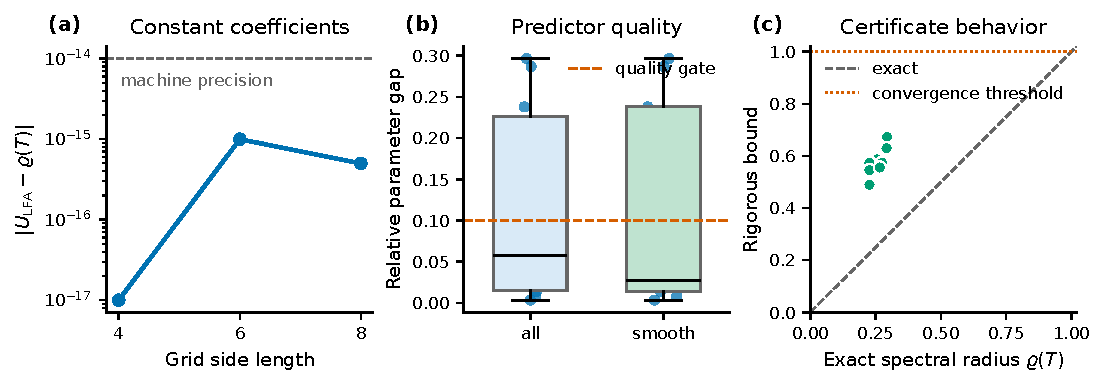
\includegraphics[width=.98\linewidth]{Fig1.pdf}
\caption{Spectral validation. \textbf{(a)}~The Fourier envelope is exact in
constant-coefficient periodic systems, with the deviation from the directly
computed radius at the level of machine precision. \textbf{(b)}~The four-corner
predictor has a small relative parameter gap in smooth variable-coefficient
cases; the dashed line is the predeclared quality gate of $0.10$.
\textbf{(c)}~The signed rate certificate is rigorous, since every point lies
above the identity line, but conservative.}
\label{fig:spectral}
\end{figure*}

\subsection{Scaling of the truncated certificate}
The rigorous truncated-kernel certificate of
Corollary~\ref{cor:truncated_kernel} produced no violation in 20 tests spanning
$8^2$ to $64^2$ grids and five truncation radii. Actual matrix-free radii were
approximately $0.269$, whereas the bounds ranged from $0.638$ to $0.681$,
corresponding to enclosure gaps of $1.38$ to $1.54$. The most expensive $64^2$
retained-radius case took $81.4$ seconds on CPU, and a relaxed $128^2$
Arnoldi certificate run did not complete within the allocated diagnostic
window. The construction therefore establishes a scalable sparse representation
in principle, but the present eigensolver and bound are not a practical
registration-time certificate. We retain it as a small-problem diagnostic and
use the predictor alone in the end-to-end timing claims.

\subsection{Controlled real-image pilot}
We next tested the multiresolution solver on a public-domain retinal image and
an unrestricted immunohistochemistry image, each subjected to three held-out
smooth known deformations. Deformation cases 1--2 were used to select a single
global manual baseline $(\rho,\alpha)=(0.1,1)$; cases 3--5 were not used for
tuning. This is a controlled real-content pilot rather than a landmark
benchmark. Against that validation-selected baseline, a single predictor
evaluation from the initial full-resolution gradient reduced the median
inner-iteration count by 44.4\%. Across five repeated, order-alternated timings
(30 paired runs), the median total-time reduction was 41.7\% (bootstrap 95\%
interval $[40.9,42.6]$\%), tuning consumed 1.58\% of proposed-method runtime,
and the median relative change in mean squared error was $-0.0068$\%. No tested
case had a nonpositive discrete Jacobian. The experiment therefore passes every
predeclared pilot gate (Table~\ref{tab:pilot}), but its two images and
controlled warps are insufficient for a clinical or benchmark claim.

\begin{table}[t]
\centering
\caption{Controlled real-image pilot against the predeclared acceptance gates;
medians over paired runs. The accuracy gate admits at most a 1\% degradation in
mean squared error.}
\label{tab:pilot}
\footnotesize
\begin{tabular}{lrr}
\toprule
Metric & Observed & Gate\\
\midrule
Inner-iteration reduction & 44.4\% & $\ge15$\%\\
Total-time reduction & 41.7\% & $\ge10$\%\\
Relative MSE change & $-0.0068$\% & $\le1$\%\\
Selection overhead & 1.58\% & $<2$\%\\
Nonpositive Jacobians & 0/6 & 0\\
\bottomrule
\end{tabular}
\end{table}

\subsection{CIMA histology landmark benchmark}
We then evaluated the public lung-lesion-3 sample distributed with the CIMA
histology-landmark repository \cite{Borovec2018}, comprising five differently
stained sections and all ten unordered image pairs. Images supplied at 5\%
scale were converted to a common structural channel by grayscale conversion,
CLAHE, Sobel magnitude, Gaussian smoothing, and fixed percentile normalization,
and were then resized to $256^2$. Manual landmarks provided at 50\% scale were
rescaled geometrically and used only for evaluation. Every method used the same
image-only robust translation initialization, selected from phase, centroid,
and clustered SIFT proposals on a $128^2$ image. A pyramid-transition safeguard
damped only the non-translational displacement when interpolation threatened
the discrete Jacobian floor.

The proposed practical policy evaluated the four-corner selector once from the
initial full-resolution gradient and reused its parameters through all levels.
The strongest fixed baseline, $(\rho,\alpha)=(0.1,1)$, had been selected on the
separate controlled real-content validation cases and was frozen before CIMA.
Across five order-alternated repetitions of all ten pairs (50 paired runs), the
predictor reduced median total runtime by 20.1\% (bootstrap 95\% interval
19.4--20.7\%), solver time by 23.5\%, and iterations by 30.1\%; selection used
1.16\% of proposed-method runtime. Median target registration error (TRE) was
$7.33$ pixels, or 2.02\% of the image diagonal, and differed by less than
$3\times10^{-5}$ pixels between the predictor and the fixed baseline
(Table~\ref{tab:cima}). The median landmark-error improvement relative to the
unregistered pairs was 36.5\%, and no global or interior nonpositive Jacobian
was observed in the final protocol. One difficult stain pair retained a TRE
above 22 pixels, identifying global initialization and cross-stain
representation, rather than ADMM convergence, as the principal failure mode.
Phase-only and unprotected pyramid runs on the same sample exposed the
initialization and upsampling failures that motivated the final shared
safeguards; those raw runs are preserved in the repository. The final CIMA
estimate is therefore a reproducible exploratory benchmark rather than a
held-out confirmatory result.

\begin{table}[t]
\centering
\caption{CIMA landmark results. Accuracy medians are taken over the ten pairs
and timing medians over 50 paired runs; the proposed method is in bold. ``BB
proxy'' is the safeguarded Barzilai--Borwein rule and ``external fixed'' is the
pair selected on the separate validation cases of Table~\ref{tab:pilot}.}
\label{tab:cima}
\footnotesize
\begin{tabular}{lrrr}
\toprule
Method & Iterations & Time (s) & TRE (px)\\
\midrule
Fixed ADMM $(1,1)$ & 1910.5 & 12.09 & 7.3310\\
Fixed oADMM $(1,1.8)$ & 1129.5 & 7.37 & 7.3308\\
Residual balancing & 1124.5 & 7.40 & 7.3310\\
BB proxy & 435.5 & 3.44 & 7.3306\\
External fixed $(0.1,1)$ & 303.5 & 2.53 & 7.3306\\
\textbf{Four-corner} & \textbf{210.0} & \textbf{2.02} & 7.3306\\
\bottomrule
\end{tabular}
\end{table}

For a diagnostic comparison in the style of Song et al. \cite{Song2024}, we
formed the exact variable-coefficient reduced operator on an $8\times8$
surrogate for every pair, optimized $\rho$ numerically with the exact
conditional $\alpha$, and then reused the result in the full solve. This
required a median of 97 spectral objective evaluations and $2.18$ seconds of
tuning. Its median full-solve iteration count was 251 versus 210 for the
four-corner predictor, and its total runtime was $4.39$ versus $2.02$ seconds,
with indistinguishable TRE. Because the $8\times8$ spectral model is a coarse
surrogate, this comparison illustrates overhead and model-transfer behavior
rather than a claim of superiority to full-resolution spectral optimization.

\subsection{FIRE retinal landmark benchmark}
We evaluated all 134 landmarked pairs in the public FIRE fundus registration
benchmark \cite{HernandezMatas2017}, comprising 14 category-A, 49 category-P,
and 71 category-S pairs. The released archive was integrity-tested with
\texttt{7z t}; images were converted to a foreground-percentile-normalized
green channel and resized to $256^2$. Supplied control points were scaled
geometrically and used only for evaluation. All methods used identical
phase-correlation initialization, three-level pyramid, objective, stopping
criteria, and a single CPU BLAS/OpenMP thread. The four-corner predictor was
evaluated once from the initial $256^2$ gradient and reused throughout the
solve. We compare against the fixed external pair $(\rho,\alpha)=(0.1,1)$
without claiming that it is a FIRE-tuned best baseline.

Across all pairs, median predictor iterations were 245 versus 412 for the fixed
pair, a paired median reduction of 39.6\%. Median total time was $4.774$ versus
$6.680$ seconds, a 34.4\% paired reduction (bootstrap 95\% interval
30.7--35.7\%), and tuning accounted for 1.2\% of proposed total time. The
safeguarded BB proxy required a median of 623.5 iterations and $9.435$
seconds; the predictor was faster on 94.0\% of pairs, with a median paired
reduction of 51.7\%. Median TRE differed from the fixed pair by
$-1.4\times10^{-5}$ pixels, with a maximum absolute difference of
$3.9\times10^{-4}$ pixels, and no method produced a nonpositive Jacobian.
Table~\ref{tab:fire} summarizes these results and Fig.~\ref{fig:fire} resolves
them per pair and per benchmark category.

\begin{table*}[t]
\centering
\caption{FIRE benchmark, 134 pairs at $256^2$, under identical initialization
and solver protocol. Medians are reported; the proposed method is in bold.
All median TRE values agree to within $4\times10^{-4}$ pixels, so the
comparison is one of cost at matched accuracy. Naming follows
Table~\ref{tab:cima}.}
\label{tab:fire}
\begin{tabular}{p{0.26\linewidth}rrrr}
\toprule
Method & Iterations & Total time (s) & TRE (px) & TRE/diagonal (\%)\\
\midrule
Fixed oADMM $(1.0,1.8)$ & 1529.5 & 23.471 & 5.50194 & 1.51971\\
Residual balancing & 1434.0 & 22.325 & 5.50211 & 1.51976\\
BB proxy & 623.5 & 9.435 & 5.50175 & 1.51966\\
External fixed $(0.1,1.0)$ & 412.0 & 6.680 & 5.50178 & 1.51967\\
\textbf{Four-corner, one-shot} & \textbf{245.0} & \textbf{4.774} & 5.50177 & 1.51966\\
\bottomrule
\end{tabular}
\end{table*}

Reported percentage reductions are medians of pairwise percentage changes and
therefore need not equal the percentage differences between the separately
reported method medians of Table~\ref{tab:fire}.

\begin{figure*}[t]
\centering
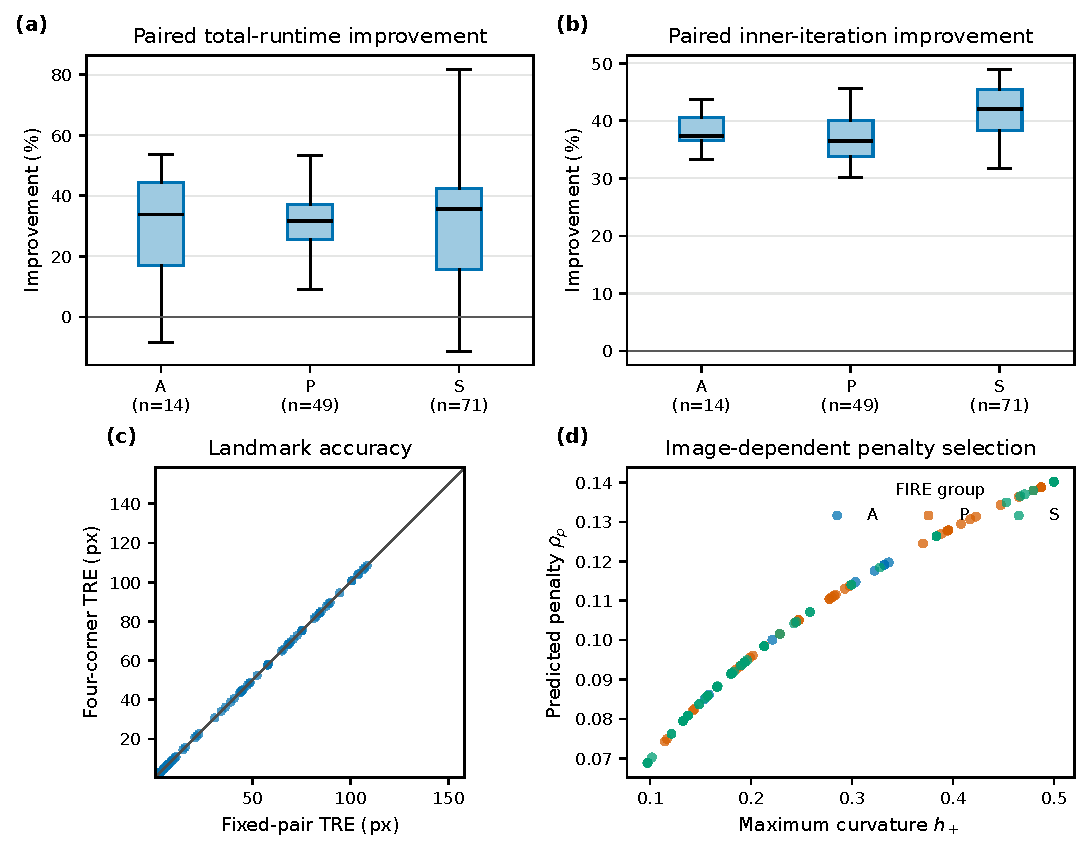
\includegraphics[width=.98\linewidth]{Fig2.pdf}
\caption{FIRE benchmark at $256\times256$ ($n=134$). \textbf{(a)}~Pairwise
total-runtime reduction of one-shot four-corner tuning relative to the
externally validation-selected fixed pair, stratified by the A, P, and S
categories. \textbf{(b)}~Corresponding inner-iteration reduction.
\textbf{(c)}~Landmark TRE for the two methods; the identity line indicates
unchanged accuracy. \textbf{(d)}~The predicted penalty $\rho_p$ varies with the
maximum data curvature $h_+$, demonstrating image-dependent tuning. Percentage
reductions are computed per pair before the category summaries.}
\label{fig:fire}
\end{figure*}

\subsection{One-shot reuse ablation}
On a balanced 18-pair FIRE ablation, retuning at every pyramid level reduced
the median inner-iteration count from 243 to 222, but increased median total
time from $2.651$ to $3.895$ seconds because of the tuning overhead. One-shot
reuse is therefore the recommended deployment policy, and it is the policy used
in all results reported above.

\section{Discussion}\label{sec:discussion}

\subsection{Convergence, prediction, and certification}
For a well-posed quadratic subproblem, Theorem~\ref{thm:basic-contraction}
already establishes convergence for every admissible pair, so tuning is a
matter of speed rather than of stability. The four-corner predictor selects a
pair expected to have a small contraction factor; it is not claimed to enclose
the exact variable-coefficient spectrum. The signed enclosures of
Section~\ref{sec:certification} are optional upper bounds on that contraction
factor and are never evaluated by the timed registration algorithm.

\subsection{Relation to adaptive and spectral tuning}
Song et al. \cite{Song2024} optimize the penalty numerically for general linear
quadratic problems and derive a conditional relaxation formula. Here, the
registration-specific rank-one geometry reduces the constant-model problem to a
finite joint selector without any repeated full-spectrum optimization. The
CIMA $8\times8$ surrogate experiment concerns overhead and model transfer only;
it is not a comparison with full-resolution spectral optimization.

\subsection{Limitations}
Outside the constant-gradient setting, the selected parameters are not claimed
to minimize the exact full spectral radius, and the finite penalty candidates
used with the signed enclosures are inherited from the local model rather than
proved to minimize those enclosures globally. Most importantly, the empirically
successful four-corner rule is predictive rather than rigorous when gradient
orientations vary.

The certificates themselves remain loose: even the Perron comparison bound
discards directional cancellation in the dense $C_G$ because it works with
block norms. Most exact spectral experiments are consequently small. The CIMA
validation uses a single five-image tissue set at reduced resolution, and the
FIRE study uses a $256^2$ CPU protocol against an externally
validation-selected fixed comparator, residual balancing, and a safeguarded
Barzilai--Borwein proxy; that proxy is not a complete reproduction of every
published adaptive ADMM variant, and the study does not establish
full-resolution clinical throughput. Finally, the theory concerns a convex
linearized subproblem and not the global convergence of the outer diffeomorphic
scheme.

\section{Conclusion}\label{sec:conclusion}

For well-posed linearized registration subproblems, all admissible ADMM
parameters are already contractive, so the practical challenge is to select a
rapidly convergent pair. We showed that rank-one data-Hessian structure reduces
the constant-model tuning problem exactly to four curvature--symbol corners,
which enables a finite algebraic one-shot predictor that requires no numerical
spectral search. On all 134 FIRE pairs at $256^2$, the predictor reduced inner
iterations by 39.6\% and median pairwise runtime by 34.4\% at essentially
unchanged landmark accuracy and with no nonpositive discrete Jacobians, and it
reduced matched-protocol runtime by 20.1\% on CIMA. Signed
variable-coefficient enclosures provide rigorous but currently conservative
optional rate bounds that the deployed algorithm does not require. Extending
the predictor to three-dimensional volumetric registration, and tightening the
enclosures so that they become usable as online tuning objectives, are the
natural directions for future work.

\backmatter

\bmhead{Supplementary information}
Supplementary Information, containing the detailed enclosure constructions,
stress tests, and full software, hardware, seed, and command details, is
supplied as Online Resource 1.

\section*{Declarations}

\begin{itemize}[leftmargin=1.2em,itemsep=2pt,topsep=2pt]
\item \textbf{Funding.} No specific funding was received for this work.
\item \textbf{Competing interests.} The authors declare no competing interests.
\item \textbf{Ethics approval and consent to participate.} Not applicable; the
study uses only publicly available, de-identified image datasets.
\item \textbf{Consent for publication.} Not applicable.
\item \textbf{Data availability.} The FIRE \cite{HernandezMatas2017} and CIMA
\cite{Borovec2018} datasets are publicly available from their original
providers. The FIRE archive is not redistributed here.
\item \textbf{Materials availability.} Not applicable.
\item \textbf{Code availability.} Source code, tests, configurations, the raw
processed JSON and CSV outputs, and the FIRE and CIMA preparation and
evaluation scripts are available at
\url{https://github.com/xhxuciedu/admm-registration}.
\item \textbf{Author contribution.} Katherine Xie and Jie Wu conducted the
research and wrote and edited the manuscript. Xiaohui Xie conceived the work
and edited the manuscript.
\end{itemize}

\begin{appendices}

\section{Proof of the Reduced Cayley Representation}\label{app:reduced}

For standard ADMM, the homogeneous updates are
\begin{equation}
v^{k+1}=P_H(w^k-u^k),
\qquad
w^{k+1}=P_G(v^{k+1}+u^k).
\end{equation}
Eliminating $v^{k+1}$ gives the state iteration
\begin{equation}
\begin{bmatrix}w^{k+1}\\u^{k+1}\end{bmatrix}
=
T_{\rho,1}
\begin{bmatrix}w^k\\u^k\end{bmatrix},
\end{equation}
where
\begin{equation}
T_{\rho,1}=
\begin{bmatrix}
P_GP_H&P_G(I-P_H)\\
(I-P_G)P_H&(I-P_G)(I-P_H)
\end{bmatrix},
\end{equation}
which factors as
\begin{equation}
T_{\rho,1}=
\begin{bmatrix}P_G\\I-P_G\end{bmatrix}
\begin{bmatrix}P_H&I-P_H\end{bmatrix}.
\end{equation}
The nonzero eigenvalues of $AB$ and $BA$ coincide, so the nonzero spectrum of
$T_{\rho,1}$ equals that of $P_HP_G+(I-P_H)(I-P_G)$. Substituting
$P_H=(I-C_H)/2$ and $P_G=(I-C_G)/2$ yields
\begin{equation}
P_HP_G+(I-P_H)(I-P_G)=\tfrac12\left(I+C_HC_G\right),
\end{equation}
which is \eqref{eq:Estandard}. The relaxed formula follows by inserting
$\widehat v^{k+1}=\alpha v^{k+1}+(1-\alpha)w^k$ from \eqref{eq:relaxed} and
collecting the same reduced state, giving
\begin{equation}
E_{\rho,\alpha}=(1-\alpha)I+\alpha E_{\rho,1}
=\left(1-\tfrac{\alpha}{2}\right)I+\tfrac{\alpha}{2}C_HC_G .
\end{equation}

\section{Proof of the Perturbation Bound}\label{app:perturbation}

For $C_A=\Id-2\rho(A+\rho\Id)^{-1}$ we have
\begin{equation}
\begin{aligned}
C_A-C_B
&=2\rho\left[(B+\rho\Id)^{-1}-(A+\rho\Id)^{-1}\right]\\
&=2\rho(A+\rho\Id)^{-1}(A-B)(B+\rho\Id)^{-1}.
\end{aligned}
\end{equation}
Since $A,B\succeq0$ imply $\norm{(A+\rho\Id)^{-1}}_2\le\rho^{-1}$, this proves
Lemma~\ref{lem:cayley_lipschitz}. Next, using $\norm{C_A}_2\le1$ for
$A\succeq0$,
\begin{equation}
\begin{aligned}
&\norm{C_HC_G-C_{\widetilde H}C_{\widetilde G}}_2\\
&\qquad\le
\norm{(C_H-C_{\widetilde H})C_G}_2
+\norm{C_{\widetilde H}(C_G-C_{\widetilde G})}_2\\
&\qquad\le\frac{2}{\rho}\left(\delta_H+\delta_G\right).
\end{aligned}
\end{equation}
Therefore
\begin{equation}
\begin{aligned}
\spr(E_{\rho,\alpha})
&\le\norm{E_{\rho,\alpha}}_2\\
&\le\norm{\widetilde E_{\rho,\alpha}}_2
+\frac{\alpha}{2}\norm{C_HC_G-C_{\widetilde H}C_{\widetilde G}}_2\\
&\le\Ulfa(\rho,\alpha)+\frac{\alpha}{\rho}\left(\delta_H+\delta_G\right),
\end{aligned}
\end{equation}
which is \eqref{eq:certified_envelope}.

\section{Proof of the Finite Candidate Sets}\label{app:candidates}

Each corner branch $\theta_c$ is rational and smooth for $\rho>0$. The
pointwise maximum can change its active branch only where two branches
intersect, which gives \eqref{eq:intersection}, and between consecutive
intersections exactly one branch is active. On such a subinterval,
differentiating $\theta(h,g;\rho)+\delta/\rho$ gives
\begin{equation}
\frac{(h+g)\left(\rho^2-hg\right)}{(\rho+h)^2(\rho+g)^2}-\frac{\delta}{\rho^2},
\end{equation}
and clearing the positive denominators yields \eqref{eq:quartic}. A global
minimum of a continuous piecewise-smooth function on a compact interval occurs
at an interval endpoint, at a nonsmooth branch intersection, or at a stationary
point of an active smooth branch, which proves
Theorem~\ref{thm:finite_candidate}.

For Theorem~\ref{thm:alpha_candidates}, note that the image of
$\theta\in[\theta_-,\theta_+]$ under $\theta\mapsto1-\alpha+\alpha\theta$ is an
interval, so the maximum absolute value occurs at one of its endpoints. The
resulting maximum of two absolute affine functions, plus a linear function of
$\alpha$, is convex and piecewise linear. Its slope changes only at the two
zero crossings, at the equioscillation intersection, and at the admissible
interval endpoints, which proves \eqref{eq:alpha_set}.

\end{appendices}

\begin{thebibliography}{99}

\bibitem{Ashburner2007}
J. Ashburner,
``A fast diffeomorphic image registration algorithm,''
\emph{NeuroImage}, vol. 38, no. 1, pp. 95--113, 2007.
DOI: 10.1016/j.neuroimage.2007.07.007.

\bibitem{Boyd2011}
S. Boyd, N. Parikh, E. Chu, B. Peleato, and J. Eckstein,
``Distributed optimization and statistical learning via the alternating direction method of multipliers,''
\emph{Foundations and Trends in Machine Learning}, vol. 3, no. 1, pp. 1--122, 2011.
DOI: 10.1561/2200000016.

\bibitem{Borovec2018}
J. Borovec, A. Mu\~noz-Barrutia, and J. Kybic,
``Benchmarking of image registration methods for differently stained histological slides,''
in \emph{Proceedings of the 2018 IEEE International Conference on Image Processing}, pp. 3368--3372, 2018.
DOI: 10.1109/ICIP.2018.8451040.

\bibitem{ChanElman1989}
T. F. Chan and H. C. Elman,
``Fourier analysis of iterative methods for elliptic problems,''
\emph{SIAM Review}, vol. 31, no. 1, pp. 20--49, 1989.
DOI: 10.1137/1031002.

\bibitem{Ghadimi2015}
E. Ghadimi, A. Teixeira, I. Shames, and M. Johansson,
``Optimal parameter selection for the alternating direction method of multipliers (ADMM): quadratic problems,''
\emph{IEEE Transactions on Automatic Control}, vol. 60, no. 3, pp. 644--658, 2015.
DOI: 10.1109/TAC.2014.2354892.

\bibitem{GiselssonBoyd2017}
P. Giselsson and S. Boyd,
``Linear convergence and metric selection for Douglas--Rachford splitting and ADMM,''
\emph{IEEE Transactions on Automatic Control}, vol. 62, no. 2, pp. 532--544, 2017.
DOI: 10.1109/TAC.2016.2564160.

\bibitem{Hering2022}
A. Hering, L. Hansen, T. C. W. Mok, et al.,
``Learn2Reg: comprehensive multi-task medical image registration challenge, dataset and evaluation in the era of deep learning,''
\emph{IEEE Transactions on Medical Imaging}, vol. 42, no. 3, pp. 697--712, 2023.
DOI: 10.1109/TMI.2022.3213983.

\bibitem{HernandezMatas2017}
C. Hern\'andez-Matas, X. Zabulis, A. Triantafyllou, P. Anyfanti, S. Douma, and A. A. Argyros,
``FIRE: fundus image registration dataset,''
\emph{Journal for Modeling in Ophthalmology}, vol. 1, no. 4, pp. 16--28, 2017.
DOI: 10.35119/maio.v1i4.42.

\bibitem{Kumar2019}
P. Kumar, C. Rodrigo, F. J. Gaspar, and C. W. Oosterlee,
``On local Fourier analysis of multigrid methods for PDEs with jumping and random coefficients,''
\emph{SIAM Journal on Scientific Computing}, vol. 41, no. 3, pp. \mbox{A1385--A1413}, 2019.
DOI: 10.1137/18M1173769.

\bibitem{MangBiros2015}
A. Mang and G. Biros,
``An inexact Newton--Krylov algorithm for constrained diffeomorphic image registration,''
\emph{SIAM Journal on Imaging Sciences}, vol. 8, no. 2, pp. 1030--1069, 2015.
DOI: 10.1137/140984002.

\bibitem{Rodrigo2017}
C. Rodrigo, F. J. Gaspar, and L. T. Zikatanov,
``On the validity of the local Fourier analysis,''
arXiv preprint arXiv:1710.00408, 2017.

\bibitem{Song2024}
J. Song, W. Lu, Y. Lei, Y. Tang, Z. Pan, and J. Duan,
``Optimizing ADMM and over-relaxed ADMM parameters for linear quadratic problems,''
\emph{Proceedings of the AAAI Conference on Artificial Intelligence}, vol. 38, no. 8, pp. 8117--8125, 2024.
DOI: 10.1609/aaai.v38i8.28651.

\bibitem{Teixeira2016}
A. Teixeira, E. Ghadimi, I. Shames, H. Sandberg, and M. Johansson,
``The ADMM algorithm for distributed quadratic problems: parameter selection and constraint preconditioning,''
\emph{IEEE Transactions on Signal Processing}, vol. 64, no. 2, pp. 290--305, 2016.
DOI: 10.1109/TSP.2015.2480041.

\bibitem{Thorley2021}
A. Thorley, X. Jia, H. J. Chang, B. Liu, K. Bunting, V. Stoll, A. de Marvao,
D. P. O'Regan, G. Gkoutos, D. Kotecha, and J. Duan,
``Nesterov accelerated ADMM for fast diffeomorphic image registration,''
in \emph{Medical Image Computing and Computer Assisted Intervention -- MICCAI 2021},
LNCS 12904, pp. 150--160, 2021.
DOI: 10.1007/978-3-030-87202-1\_15.

\bibitem{Vercauteren2009}
T. Vercauteren, X. Pennec, A. Perchant, and N. Ayache,
``Diffeomorphic demons: efficient non-parametric image registration,''
\emph{NeuroImage}, vol. 45, no. 1, suppl. 1, pp. S61--S72, 2009.
DOI: 10.1016/j.neuroimage.2008.10.040.

\bibitem{WienandsJoppich2005}
R. Wienands and W. Joppich,
\emph{Practical Fourier Analysis for Multigrid Methods}.
Boca Raton, FL: Chapman \& Hall/CRC, 2005.

\bibitem{Wohlberg2017}
B. Wohlberg,
``ADMM penalty parameter selection by residual balancing,''
arXiv preprint arXiv:1704.06209, 2017.

\bibitem{Xu2017}
Z. Xu, M. A. T. Figueiredo, and T. Goldstein,
``Adaptive ADMM with spectral penalty parameter selection,''
in \emph{Proceedings of the 20th International Conference on Artificial Intelligence and Statistics},
PMLR, vol. 54, pp. 718--727, 2017.

\end{thebibliography}

\end{document}
